% !TeX spellcheck = de_DE

\section{Ergebnisse} \label{audiotracer_results}
Dieses Kapitel listet einige Testreihen mit verschiedenen Audiodateien auf. Für jede Audiodatei werden Tests mit zwei verschiedenen Schwellwerten an Eingabesamples und diese jeweils für beide AudioTracer-Module wiederholt.
Die Testreihen sind wie folgt einzuordnen:
\begin{table}[h!]
	\centering
	\begin{tabular}{|c | c | c | c|}
		\hline
		Testreihe & \#Samples & \#Kanäle & Modul(AudioTracer)\\
		\hline\hline
		1		&	5000	&	2	&	C \\
		2		&	5000	&	2	&	Python \\
		3		&	25000	&	2	&	C \\
		4		&	25000	&	2	&	Python \\
		5		&	5000	&	4	&	C \\
		6		&	5000	&	4	&	Python \\
		7		&	25000	&	4	&	C \\												
		8		&	25000	&	4	&	Python \\
		\hline	
		
	\end{tabular}	
\end{table}

Die Testreihen für die Module werden in den nächsten beiden Sektionen getrennt dargelegt.
Es werden zwei verschiedene Audiodateien mit zwei bzw. vier Audiokanälen verwendet.
Die Dateien bestehen aus je einer Sinuskurve für jeden Audiokanal mit bekannter Frequenz. Die Frequenzen sind in folgender Übersicht aufgelistet:

\begin{table}[h!]
	\centering
	\begin{tabular}{|c | c | c | c | c |}		
		\hline
		Datei/Kanal\# & 1 & 2 & 3 & 4\\
		\hline\hline
		2channelKnownFreqTest.wav		&	300Hz & 40Hz & - & - \\
		4channelKnownFreqTest.wav		&	30Hz  &	100Hz	&	160Hz & 210Hz \\
		\hline	
		
	\end{tabular}	
\end{table}

\newpage

\subsection{AudioTracer C}
Die Auswertung für das AudioTracer(C)-Modul thematisiert die Testreihen 1, 3, 5 und 7.
Dabei werden die Reihen mit gleicher Anzahl von Audiokanälen nebeneinander abgebildet.
Hierbei sei zu bemerken, dass die Ergebnisse eine Momentaufnahme einer Live-Visualisierung darstellen. Jeweils ein Block der fouriertransformierten Daten der Größe \#Samples wird hier abgebildet. 

\paragraph{Testreihe 1 und 3}
-
\begin{table}[h!]
	\centering
	\begin{tabular}{|c | c | c | c | c |}		
		\hline
		Testreihe/erwartet & 300Hz & 40Hz \\
		\hline\hline
		1		&	299,88Hz, -299,88Hz & 44,1Hz, -44,1Hz \\
		3		&	299,88Hz, -299,88Hz  &	38,808Hz, -38,808Hz	\\
		\hline	
	\end{tabular}	
\end{table}

Die negativen Frequenzen werden zukünftig nicht mehr mit aufgezählt, da diese rechnerisch durch die Fouriertransformation gleich sind. Aus Gründen der Vervollständigung wurden diese hier mit angegeben und sind implizit bei den restlichen Testreihen zu erwarten.

\begin{figure}[h!]
	\centering      
	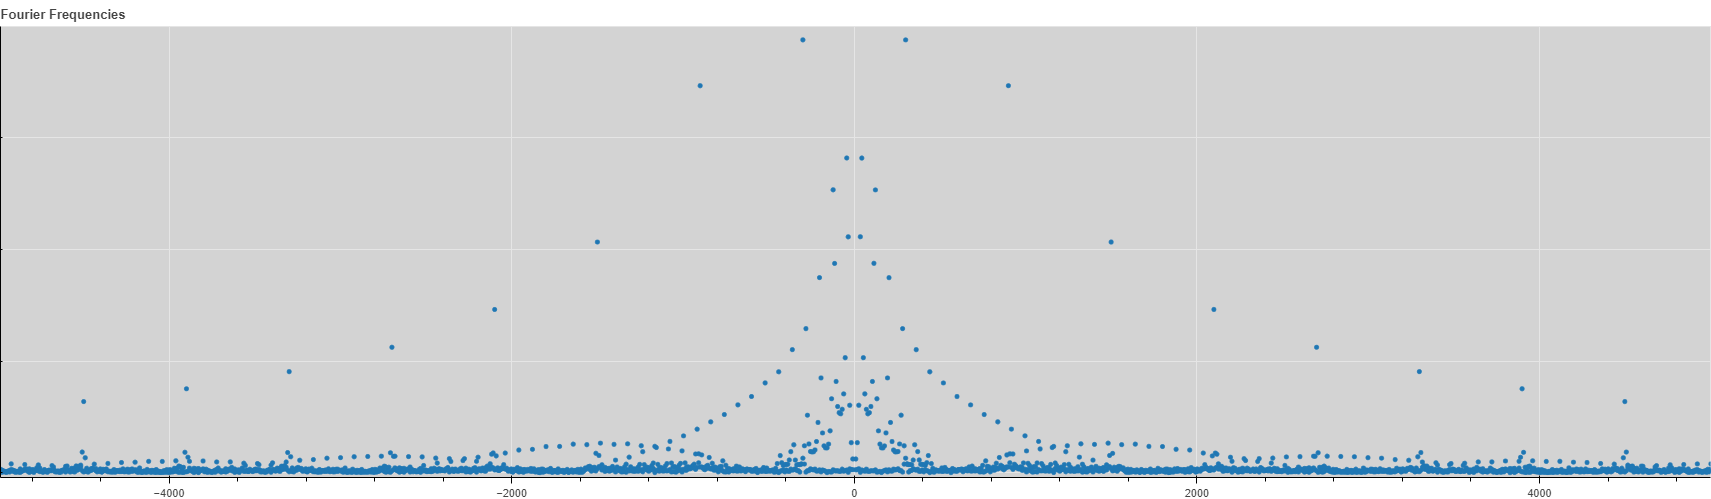
\includegraphics[scale=0.34]{results/test1.png}
	\caption{Test 1}
	\label{fig:test1}
\end{figure}

\begin{figure}[h!]
	\centering      
	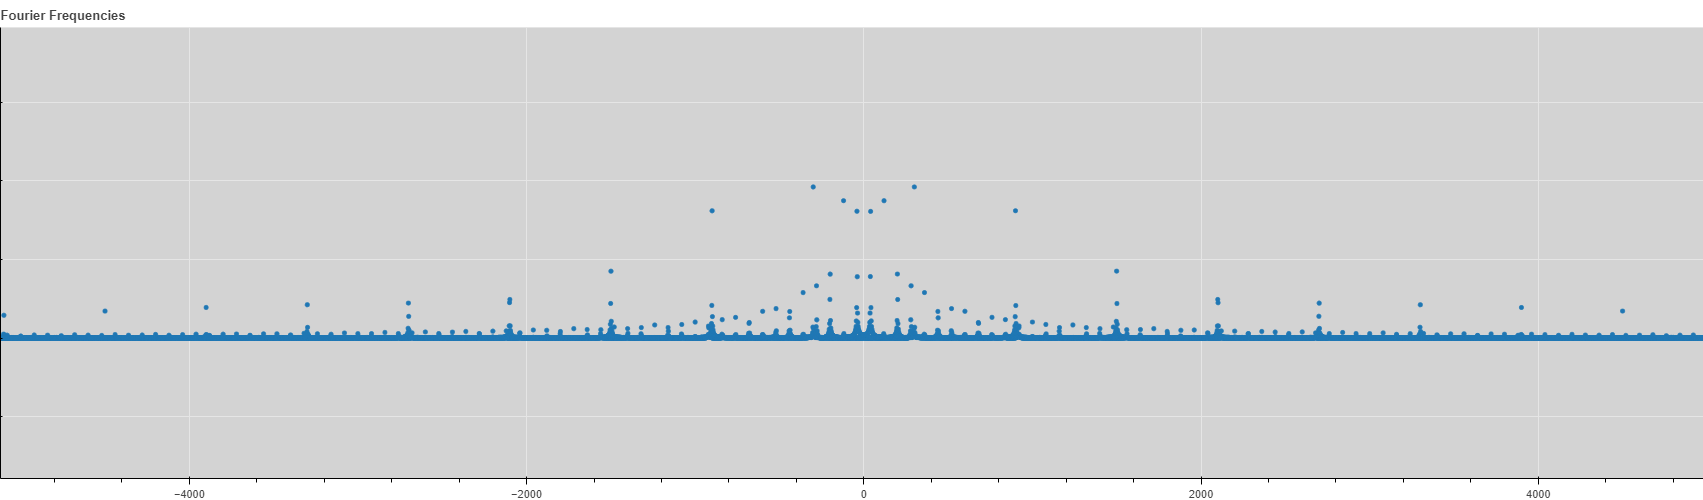
\includegraphics[scale=0.34]{results/test3.png}
	\caption{Test 3}
	\label{fig:test3}
\end{figure}

\newpage

\paragraph{Testreihe 5 und 7}

-
\begin{table}[hbt]
	\centering
	\begin{tabular}{|c | c | c | c | c |}		
		\hline
		Testreihe/erwartet & 30Hz & 100Hz & 160Hz & 210Hz\\
		\hline\hline
		5		&	26,46Hz & 97,02Hz & 158,76Hz & 211,68Hz \\
		7		&	29,988Hz & 100,548Hz & 160,524Hz & 209,916Hz \\
		\hline	
	\end{tabular}	
\end{table}

\begin{figure}[hbt]
	\centering      
	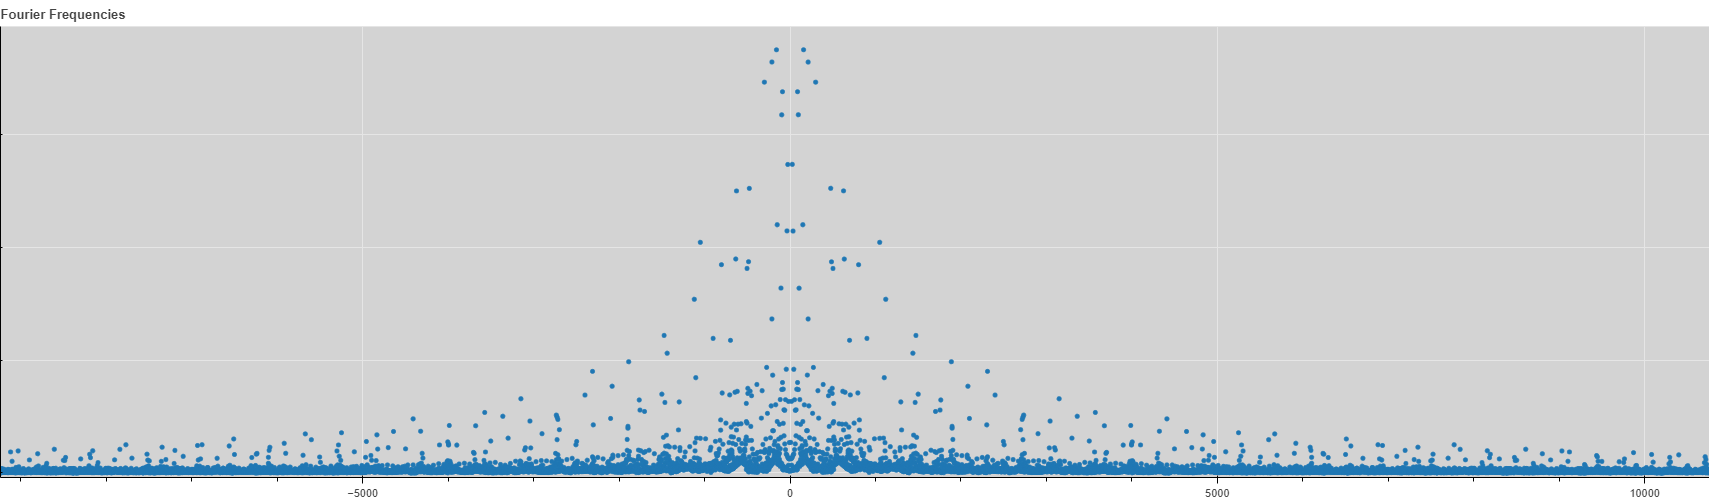
\includegraphics[scale=0.34]{results/test5.png}
	\caption{Test 5}
	\label{fig:test5}
\end{figure}

\begin{figure}[hbt]
	\centering      
	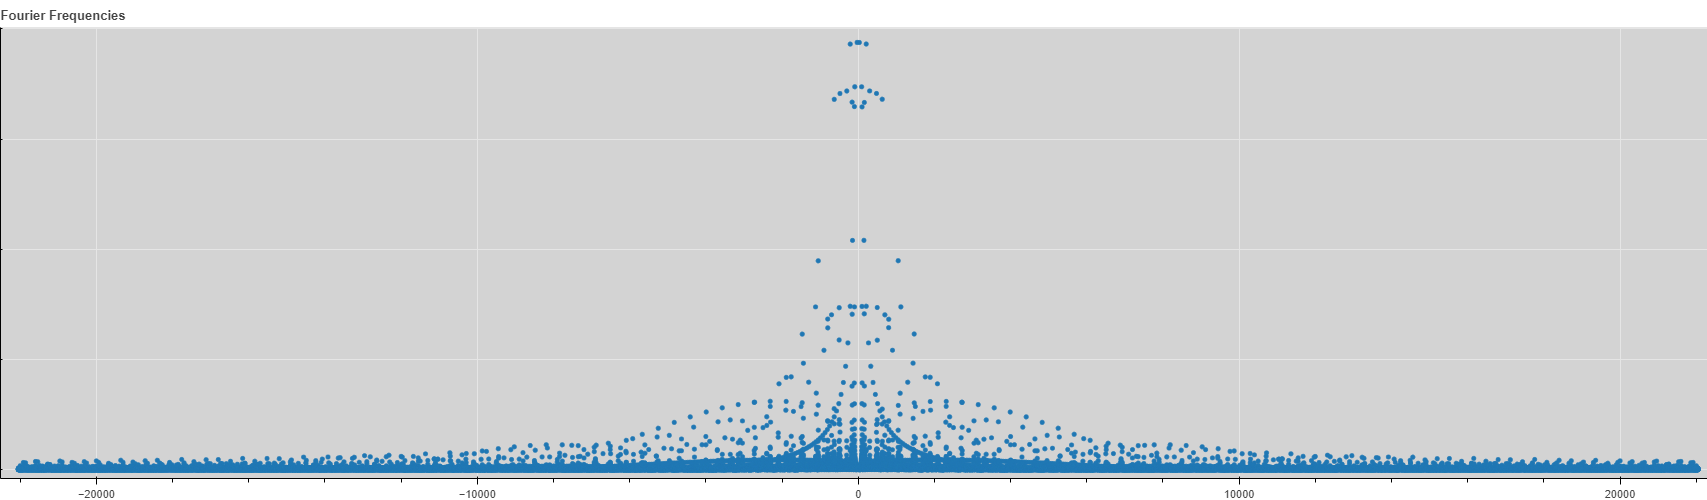
\includegraphics[scale=0.34]{results/test7.png}
	\caption{Test 7}
	\label{fig:test7}
\end{figure}

\newpage
\subsection{AudioTracer Python}

\paragraph{Testreihe 2 und 4}
-

\begin{table}[h!]
	\centering
	\begin{tabular}{|c | c | c | c | c |}		
		\hline
		Testreihe/erwartet & 300Hz & 40Hz \\
		\hline\hline
		2		&	299,88Hz & 44,1Hz \\
		4		&	299,88Hz & 40,572Hz	\\
		\hline	
	\end{tabular}	
\end{table}

\begin{figure}[h!]
	\centering      
	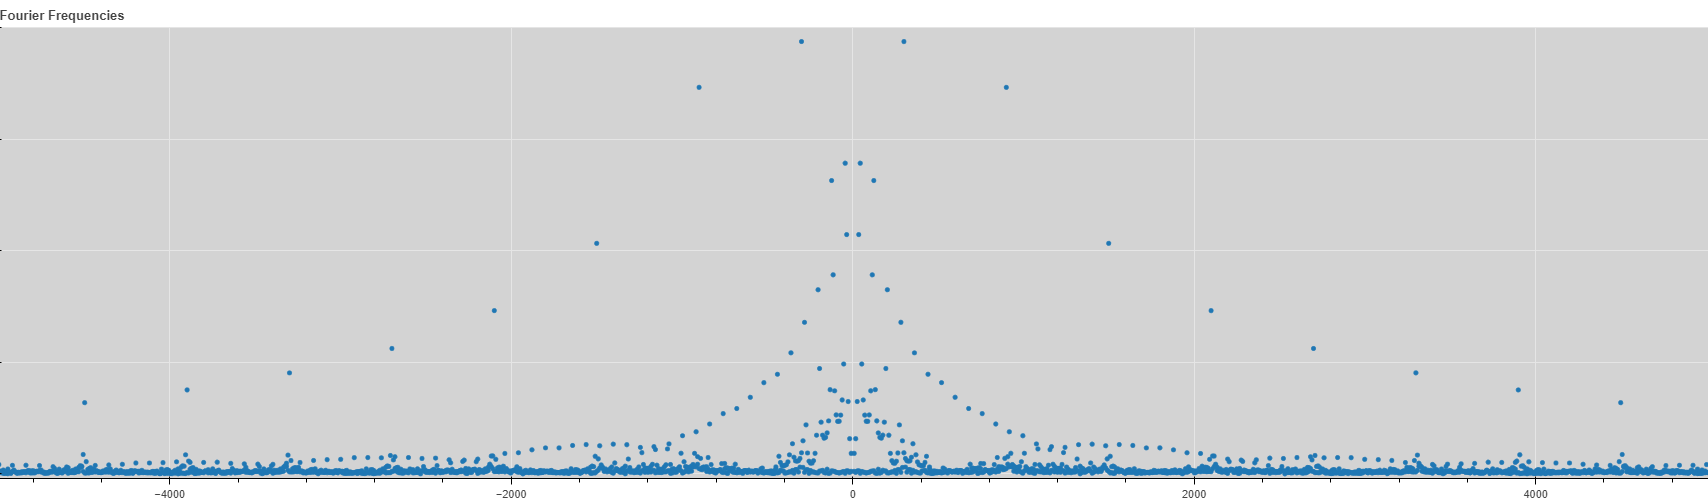
\includegraphics[scale=0.34]{results/test2.png}
	\caption{Test 2}
	\label{fig:test2}
\end{figure}

\begin{figure}[h!]
	\centering      
	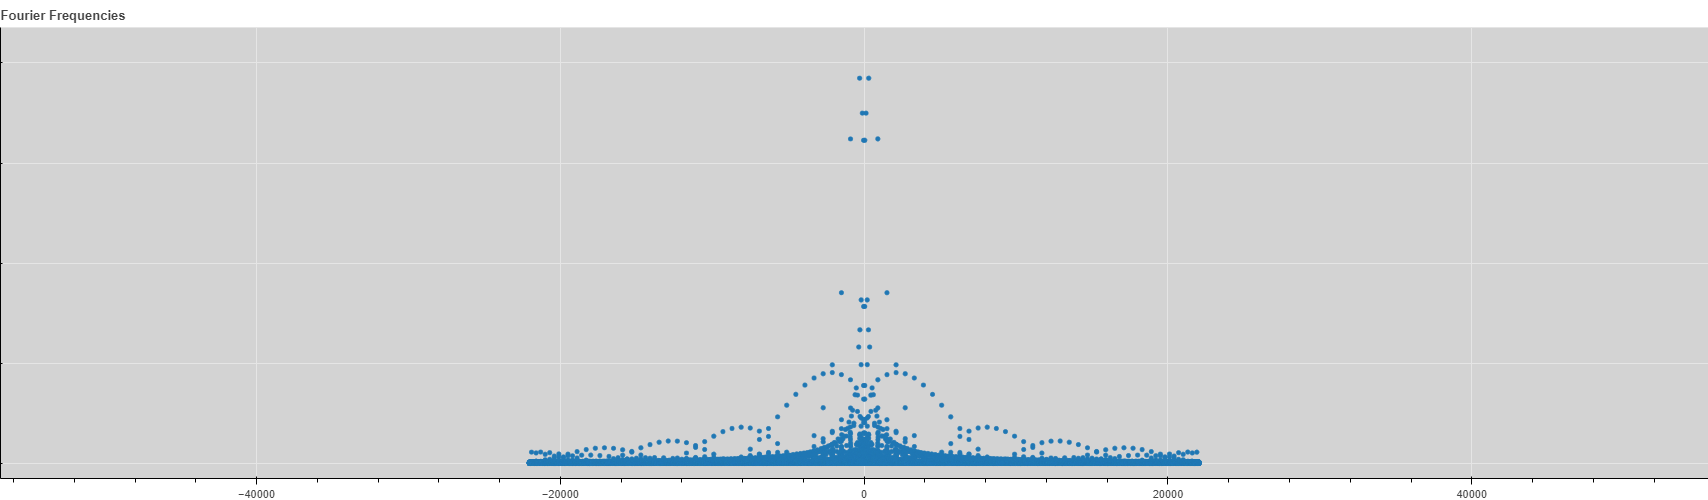
\includegraphics[scale=0.34]{results/test4.png}
	\caption{Test 4}
	\label{fig:test4}
\end{figure}

\newpage

\paragraph{Testreihe 6 und 8}
-

\begin{table}[h!]
	\centering
	\begin{tabular}{|c | c | c | c | c |}		
		\hline
		Testreihe/erwartet & 30Hz & 100Hz & 160Hz & 210Hz\\
		\hline\hline
		5		&	26,46Hz & 97,02Hz & 158,76Hz & 211,68Hz \\
		7		&	29,988Hz & 100,548Hz & 160,524Hz & 209,916Hz \\
		\hline	
	\end{tabular}	
\end{table}


\begin{figure}[h!]
	\centering      
	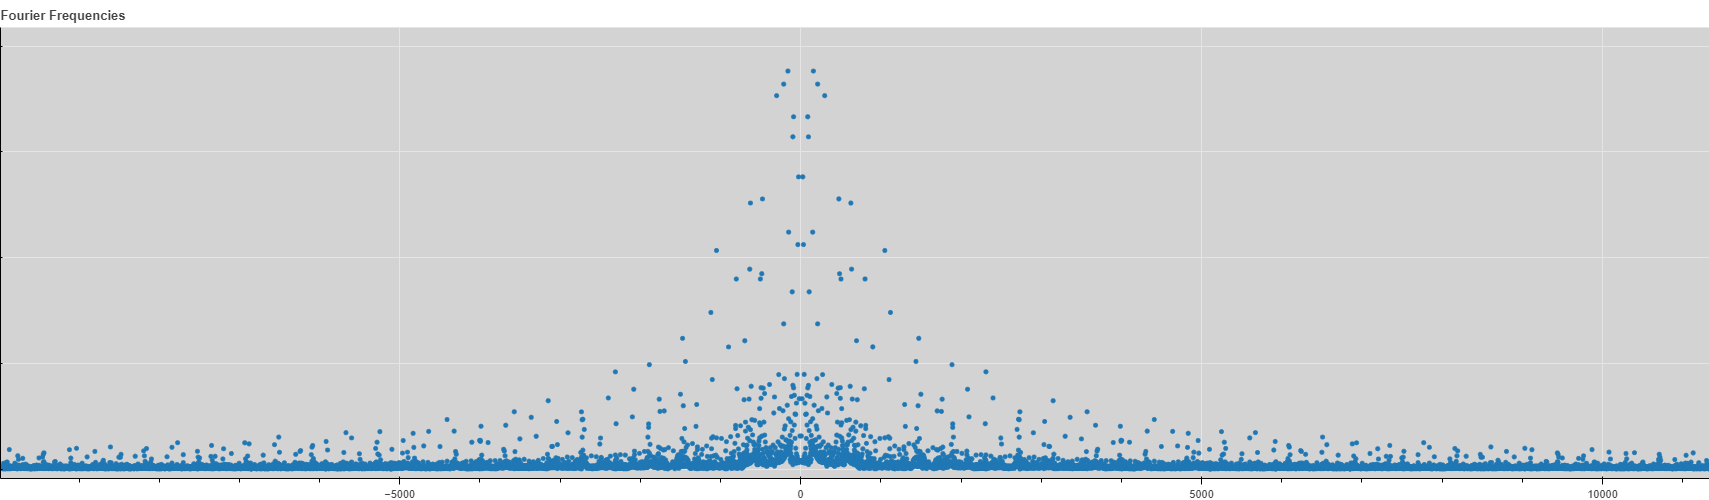
\includegraphics[scale=0.34]{results/test6.png}
	\caption{Test 6}
	\label{fig:test6}
\end{figure}

\begin{figure}[h!]
	\centering      
	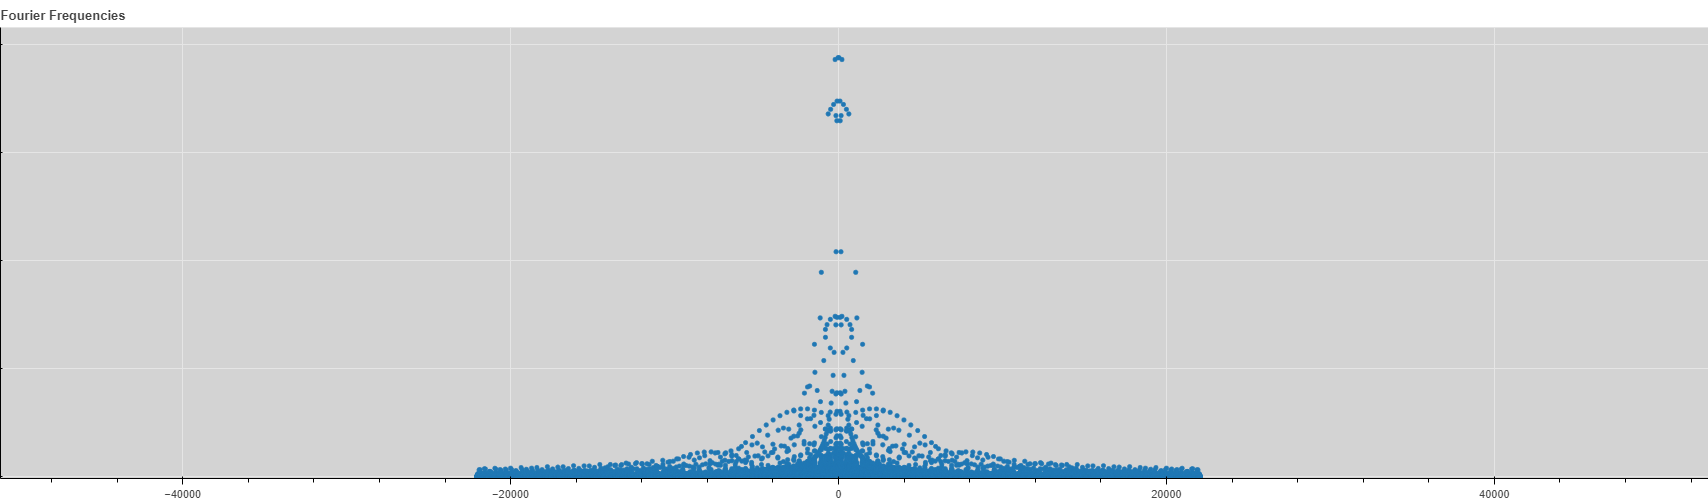
\includegraphics[scale=0.34]{results/test8.png}
	\caption{Test 8}
	\label{fig:test8}
\end{figure}

\newpage

\subsection{Vergleich der Testreihen}

Das Ziel der Anwendung einer Fouriertransformation ist eine möglichst genaue Extraktion der einzelnen Frequenzen, die zum angegebenen Teilbereich gehören.
Erkennbar ist, dass die ermittelten Frequenzen nicht genau die erwarteten Hertz-Zahlen erreichen. Ein genereller Trend ist bei den Testreihen 5, 7 und 6, 8 mit vier Audiokanälen zu erkennen. Hier werden die Ergebnisse mit steigender Sample Anzahl genauer. Die Abweichungen liegen den Reihen 7 und 8 bei 0,012 bis 0,84 Hz. Die Testreihen 5 und 6 weisen einen Fehlerbereich von 1,24 bis 3,54Hz auf, was die Eingangsthese unterstützt.

Bei den Testreihen mit nur zwei Audiokanälen ist eine ähnliche Tendenz zu erkennen, jedoch treten hier folgende Anomalien auf: Der mit 300Hz zu erwartende Wert weist bei allen vier teilhabenden Testreihen (1, 3, 2 und 4) denselben Wert von 299,88Hz auf. Bei zu erwartenden 40Hz im zweiten Audiokanal liegen die Testreihen mit 5000 Audiosamples mit 4,1Hz deutlich über denen mit 25000 Audiosamples (1,192Hz und 0.572Hz). Außerdem sind die Ergebnisse zwischen C- und Python-Modul unterschiedlich, was bei den Testreihen mit vier Audiokanälen nicht der Fall ist. Die Annahme liegt nahe, dass bedingt durch die Momentaufnahme der Ausgabe ein \enquote{ungünstiger} Moment aufgenommen wurde und somit die Daten ungenau werden. Der Unterschied zwischen zwei Frequenzen fällt bereits bei 1Hz Differenz durch genaues Hinhören auf.

Allgemein sticht jedoch heraus, dass die Erhöhung der Eingabesamples für eine genauere Berechnung der Fourierfrequenzen sorgt. 




%\subsection{Parallele Transformation und herkömmliche}

